\documentclass[11pt,a4paper]{article}
\usepackage[margin=2.4cm]{geometry}
\usepackage{booktabs}
\usepackage{array}
\usepackage{amsmath,amssymb}
\usepackage[table]{xcolor}
\usepackage{ragged2e}
\usepackage{pifont}
\usepackage{enumitem}
\usepackage{pdflscape}
\usepackage[expansion=false]{microtype}
\usepackage[T1]{fontenc}
\usepackage{tikz}
\usetikzlibrary{positioning,arrows,calc}
\usepackage[colorlinks=true,linkcolor=blue!50!black]{hyperref}

\newcommand{\yes}{\textcolor{green!45!black}{\ding{51}}}
\newcommand{\yy}{\textcolor{green!45!black}{\ding{51}\ding{51}}}
\newcommand{\no}{\textcolor{red!70!black}{\ding{55}}}
\newcommand{\nn}{\textcolor{red!70!black}{\ding{55}\ding{55}}}
\newcommand{\marg}{\textcolor{orange!80!black}{$\sim$}}
\newcolumntype{L}[1]{>{\RaggedRight\arraybackslash}p{#1}}
\newcolumntype{C}[1]{>{\Centering\arraybackslash}p{#1}}
\newcommand{\Aom}{A_\Omega}

\title{\vspace{-1.5em}One sigmoid, several doors\\
\large What is lumped into a neural-mass transfer function, and why TI enters by a different one}
\author{}
\date{\today}

\begin{document}
\maketitle
\vspace{-2.5em}

\begin{abstract}
\noindent Neural-mass models pass every input through a single kernel before it reaches the sigmoid,
because they were built for synaptic drive. An applied electric field does not use that route: it
polarizes membrane directly, including at the spike-initiation site, skipping the synapse and most of
the cable. Writing the sigmoid's argument as a \emph{sum of separately filtered entry points} --- one
per physical route in --- costs one equation, changes nothing else in the model, and resolves the
kHz-carrier problem in temporal interference (TI): at kHz all the slow doors are shut and only the axon
initial segment (AIS) is still open. The same structure explains why the TI response is controlled by
the slow input (which sets the operating point) even though the slow input cannot carry the carrier,
and it locates the one remaining lumped assumption --- that the sigmoid is static --- as the true
frequency ceiling of the mechanism.
\end{abstract}

\section{The problem, stated plainly}

Section 2.6 as drafted makes three moves. It notes that the membrane low-passes the field before the
spike nonlinearity; it evaluates that filter with the somatic time constant, $\tau_m\sim16$\,ms,
finding $|H_m|^2\sim10^{-4}$ at 1\,kHz and concluding that somatic demodulation is dead; and it escapes
by putting the nonlinearity at a fast element instead, letting the population amplify the recovered
envelope near a Hopf bifurcation, $G\sim1/\gamma$.

The escape is presented as a parameter swap, $\tau_m\rightarrow\tau_f$. It is not. In the second move
the demodulator is the \emph{population} sigmoid; in the third it is a \emph{single-cell} conductance
nonlinearity, and the population sigmoid has quietly been demoted to a linear transducer. A reader
carrying Eq.~(18) forward is left holding a population $\sigma''$ evaluated behind a single-cell filter.

The resolution is not to choose between them. It is to notice that the sigmoid was never the problem.

\section{One sigmoid, several doors}

\subsection{What the standard kernel lumps}

In Jansen--Rit the chain is
\[
\text{presynaptic rate }\phi
\;\longrightarrow\;
h(t)=A\,a\,t\,e^{-at}
\;\longrightarrow\;
v
\;\longrightarrow\;
\sigma(v)
\;\longrightarrow\;
\text{output rate}.
\]
The kernel $h$ lumps together \emph{everything} between a presynaptic spike and its effect at the place
where spikes are made: transmitter release, receptor kinetics, dendritic cable, somatic membrane. Its
corner, $1/a\sim10$\,ms $\Rightarrow$ $\sim$16\,Hz, is set by the slowest link in that chain. For
synaptic input this is entirely correct --- a presynaptic spike really does have to traverse all of it.

The error is to conclude that \emph{every} input must traverse all of it. An applied electric field does
not. It polarizes membrane directly and everywhere at once, including at the spike-initiation site. It
skips the synapse, the receptor, and most of the cable.

Note also what the sigmoid's \emph{argument} is. In QIF, $v$ is defined operationally as whatever
voltage runs to threshold and resets --- the spike-generating variable, anatomically the AIS. In
Jansen--Rit, $\sigma$ is likewise defined by what it does, mapping a potential to a firing rate, so its
argument is the spike-initiating potential by construction. Both models are already AIS-referenced.
There is \emph{no filter between $v$ and $\sigma$}; all the filtering is in $h$, upstream.

\subsection{The model}

So write the argument of $\sigma$ as a sum over entry points, each with its own kernel:
\begin{equation}
\boxed{\;v(t)=\sum_k \bigl(h_k * u_k\bigr)(t),
\qquad r(t)=\sigma\bigl(v(t)\bigr)\;}
\label{eq:doors}
\end{equation}
with $u_k$ the physical input at door $k$ and $h_k$ its transfer function. Nothing else in the model
changes: $\sigma$ keeps its shape, its argument, and its curvature.

\begin{table}[h]
\centering
\small
\renewcommand{\arraystretch}{1.2}
\begin{tabular}{@{}c L{4.6cm} L{2.3cm} L{2.6cm} c L{3.2cm}@{}}
\toprule
$k$ & Door & Input $u_k$ & Coupling $\lambda_k$ & Corner of $h_k$ & Dominates when \\
\midrule
1 & synapse $\rightarrow$ dendrite $\rightarrow$ soma & presynaptic rate $\phi$ & --- & $\sim$16\,Hz & normal operation \\
2 & field $\rightarrow$ soma / dendrite & field $\varepsilon$ & large (whole-cell dipole) & $\sim$10\,Hz & DC and slow tES \\
\rowcolor{green!8}
3 & \textbf{field $\rightarrow$ AIS} & field $\varepsilon$ & moderate, $\lambda(\omega)$ & $\sim$800\,Hz & \textbf{kHz carriers: TI} \\
4 & field $\rightarrow$ presynaptic terminal & field $\varepsilon$ & small & 1--3\,kHz & very high carriers \\
\bottomrule
\end{tabular}
\caption{Entry points into the same state variable. Corners are order-of-magnitude.}
\label{tab:doors}
\end{table}

Two things follow immediately.

\textbf{The same physical field enters through more than one door.} At DC, door 2 wins, because the
whole-cell dipole gives it the largest $\lambda$. At kHz, doors 1 and 2 are shut and door 3 is the only
one still open. This is one cell and one field: which door dominates is set by \emph{frequency}. It is
also why the tES literature is soma- and dendrite-centered and why TI cannot be.

\textbf{The doors are in parallel, not in series.} That is the entire content of the proposal. The
standard picture puts every input behind one door, in series with the slowest link in the chain.

\begin{figure}[h]
\centering
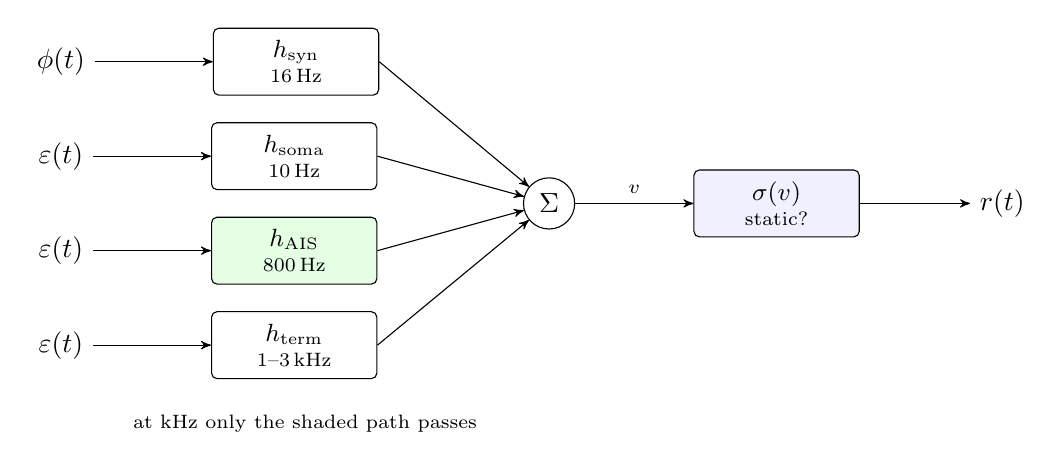
\begin{tikzpicture}[
  box/.style={draw,rounded corners=2pt,minimum width=2.1cm,minimum height=0.85cm,align=center,font=\small},
  sum/.style={draw,circle,minimum size=0.65cm,inner sep=0pt},
  >=stealth', node distance=0.55cm and 1.5cm]

\node (u1) at (0,2.4) {$\phi(t)$};
\node (u2) at (0,1.2) {$\varepsilon(t)$};
\node (u3) at (0,0.0) {$\varepsilon(t)$};
\node (u4) at (0,-1.2) {$\varepsilon(t)$};

\node[box,right=of u1] (h1) {$h_{\rm syn}$\\[-2pt]{\scriptsize 16\,Hz}};
\node[box,right=of u2] (h2) {$h_{\rm soma}$\\[-2pt]{\scriptsize 10\,Hz}};
\node[box,right=of u3,fill=green!10] (h3) {$h_{\rm AIS}$\\[-2pt]{\scriptsize 800\,Hz}};
\node[box,right=of u4] (h4) {$h_{\rm term}$\\[-2pt]{\scriptsize 1--3\,kHz}};

\node[sum] (S) at (6.2,0.6) {$\Sigma$};
\node[box,right=1.5cm of S,fill=blue!6] (sig) {$\sigma(v)$\\[-2pt]{\scriptsize static?}};
\node[right=1.4cm of sig] (out) {$r(t)$};

\foreach \i in {1,2,3,4}{\draw[->] (u\i) -- (h\i);}
\foreach \i in {1,2,3,4}{\draw[->] (h\i.east) -- (S);}
\draw[->] (S) -- node[above,font=\scriptsize]{$v$} (sig);
\draw[->] (sig) -- (out);

\node[font=\scriptsize,align=center] at (3.1,-2.2)
  {at kHz only the shaded path passes};
\end{tikzpicture}
\caption{Entry points in parallel. Each door carries the same state variable but with its own transfer
function; the nonlinearity sees only the sum.}
\label{fig:doors}
\end{figure}

\subsection{Why the carrier now survives: three lines}

Split $v$ into what is slow and what is at the carrier:
\begin{equation}
v(t)=v_{\rm slow}(t)+a(t)\cos\omega_c t,
\end{equation}
where $v_{\rm slow}$ is everything arriving through doors 1 and 2 (synaptic drive plus any DC field
polarization), and $a(t)\cos\omega_c t$ is what door 3 lets through. In TI the two beating carriers make
$a$ time-dependent, $a(t)=a_0\bigl[1+m\cos\Omega t\bigr]$ to first order, with $\Omega$ the envelope
frequency.

Because $\sigma$ is static, expand about $v_{\rm slow}$:
\begin{equation}
r(t)=\underbrace{\sigma(v_{\rm slow})}_{\text{ordinary rate}}
\;+\;\underbrace{\sigma'(v_{\rm slow})\,a\cos\omega_c t}_{\text{at kHz: network cannot follow}}
\;+\;\underbrace{\tfrac12\sigma''(v_{\rm slow})\,a^2\cos^2\!\omega_c t}_{\text{the demodulator}}
\;+\;\cdots
\label{eq:taylor}
\end{equation}
The third term is the whole mechanism. Using $\cos^2\theta=\tfrac12(1+\cos2\theta)$,
\begin{equation}
\tfrac12\sigma''a^2\cos^2\!\omega_ct
=\underbrace{\tfrac14\sigma''\,a(t)^2}_{\textbf{baseband}}+\tfrac14\sigma''a^2\cos2\omega_ct ,
\qquad
\tfrac14\sigma''a_0^2\bigl[1+m\cos\Omega t\bigr]^2
\;\supset\;
\tfrac12\sigma''a_0^2\,m\cos\Omega t .
\end{equation}
That last term is the TI signal. It sits at $\Omega\approx10$\,Hz, and --- this is the point --- nothing
upstream can attenuate it, because it did not exist upstream. It was created \emph{after} every filter
that could have killed it. Whatever comes next (synaptic kinetics, dendritic cable, the network's own
dynamics) sees only $\Omega$, which is inside its passband, and the population near a Hopf bifurcation
amplifies it by $G\sim1/\gamma$.

Equation~(18) is therefore not wrong. It is the response computed through \emph{door 2}, which is the
wrong door for TI.

\subsection{The slow input still controls everything}

In Eq.~\eqref{eq:taylor}, $\sigma''$ is evaluated at $v_{\rm slow}$. So the slow doors, which cannot
carry the carrier at all, nevertheless set where on the sigmoid the population sits, and hence the size
--- and sign --- of the response. This is exactly the falsifiable handle the introduction claims, now
with a mechanism attached:
\begin{itemize}[leftmargin=1.4em,itemsep=1pt,topsep=2pt]
\item anything shifting $v^*$ --- neuromodulation, attention, arousal, psychedelics, interneuron
      dysfunction --- rescales the TI response through $\sigma''(v^*)$;
\item because $\sigma''$ vanishes at the inflection of $\sigma$ and reverses beyond it, the response
      \emph{flips sign} when $v^*$ crosses that point. In the exact mean-field treatment of \S5 this
      crossing has a closed form, $\bar\eta+I=\Delta/\sqrt3$.
\end{itemize}
Note the asymmetry this predicts: a slow input can gate a fast one, but not conversely.

\subsection{A degeneracy that TI breaks}

Why has none of this mattered before? Because at low frequency the AIS and the soma are electrotonically
one compartment, so ``somatic potential'' and ``spike-initiating potential'' are the same number, and
doors 2 and 3 are indistinguishable. The identification of the neural-mass state variable is
\emph{degenerate} at DC. It stops being degenerate at kHz, where the space constant has contracted,
\begin{equation}
\lambda(\omega)=\lambda_0\bigl(1+\omega^2\tau_m^2\bigr)^{-1/4},
\label{eq:lambda}
\end{equation}
by roughly tenfold at 1\,kHz with $\tau_m=16$\,ms --- down to tens of \textmu m, comparable to the AIS
length itself. TI is thus the experiment that makes the identification determinate. That is a more
interesting claim than a filter argument, and worth making explicitly.

\subsection{What is still lumped}

Two assumptions survive Eq.~\eqref{eq:doors}, and both have a validity bandwidth.

\emph{(a) Each $h_k$ lumps a chain of stages.} This is fine, and it is the point: each is valid below
its own corner, and the corners differ by two orders of magnitude, which is what makes the doors
distinguishable.

\emph{(b) $\sigma$ is static.} This is the remaining lump and it has the shortest validity. A static
$\sigma$ is the $\tau_{\rm gate}\rightarrow0$ idealization of an ensemble spike-initiation
nonlinearity whose Na$_{\rm v}$ activation gate has $\tau\approx0.1$--$0.2$\,ms, i.e.\ a corner around
1\,kHz. Above it, $\sigma''$ is itself frequency-dependent and Eq.~\eqref{eq:taylor} acquires a factor
$|H_{\rm gate}(\omega_c)|^2$. \textbf{This, not the membrane, is the true frequency ceiling of TI} ---
and it is a prediction rather than a caveat.

\subsection{What to measure}

Sweeping the carrier $f_c$ at fixed envelope frequency $\Omega$ and fixed field magnitude should give
\begin{equation}
\Aom(f_c)\;\propto\;\bigl|H_{\rm AIS}(\omega_c)\bigr|^2\,\bigl|H_{\rm gate}(\omega_c)\bigr|^2
\;\times\;\tfrac12\sigma''(v^*)\,G(\gamma),
\end{equation}
i.e.\ a product of two Lorentzian-like roll-offs with corners near 800\,Hz and 1--3\,kHz, rather than the
single 10\,Hz corner that door 2 would give. The carrier sweep therefore \emph{measures which door is
open}, and any departure from this shape is evidence of a door not in Table~\ref{tab:doors}. Repeating
the sweep under a manipulation that shifts $v^*$ should rescale the whole curve without moving its
corners --- a clean separation of the access factor from the demodulation factor.

\section{Which nonlinearity, physically}

Equation~\eqref{eq:doors} says the demodulator must satisfy three independent requirements.
\textbf{A --- access:} the carrier must reach it, $\tau_{\rm acc}\lesssim1/\omega_c$, with quadratic
penalty $|H_{\rm acc}|^2$. \textbf{G --- gate:} the nonlinearity must itself rectify at kHz,
$\tau_{\rm gate}\lesssim1/\omega_c$. \textbf{R --- readout:} the $\Omega$ product must be injected where
the slow network integrates. Table~\ref{tab:cands} applies all three to every candidate from soma to
synapse.

Exactly two rows pass: the AIS, and marginally the presynaptic Ca$_{\rm v}$. Rows 8 and 10 --- the
Hill-coefficient release step and the population Hopf --- are the \emph{gain chain}, not the detector,
which is worth saying out loud since row 8 is the steepest nonlinearity in the cell. Rows 1--3 all fail
for the same reason and can collapse into one paragraph.

\begin{landscape}
\begin{table}
\centering
\renewcommand{\arraystretch}{1.25}
\setlength{\tabcolsep}{4pt}
\footnotesize
\begin{tabular}{@{}c L{3.5cm} C{2.5cm} C{2.6cm} L{2.0cm} L{3.9cm} L{4.4cm}@{}}
\toprule
\# & \textbf{Site / mechanism} & \textbf{A}: $\tau_{\rm acc}$, $|H|^2$ & \textbf{G}: $\tau_{\rm gate}$, kHz? & \textbf{Curvature} & \textbf{R}: slow-network readout & \textbf{Verdict} \\
\midrule
1 & Soma --- population sigmoid $\sigma(v)$ & 10--30\,ms \newline $\sim10^{-4}$ & static (mean field) & high ($\sigma''$) & \yes\ rate code & \no\ \textbf{fails A} --- the Eq.~(18) baseline \\
2 & Dendrite --- NMDA spike / Ca$^{2+}$ plateau & 10--30\,ms \newline $\sim10^{-4}$ & 50--100\,ms \quad \nn & very high & \yes & \nn\ \textbf{fails A and G} \\
3 & Soma/dendrite --- persistent Na$^+$ ($I_{\rm NaP}$) & 10--30\,ms \newline $\sim10^{-4}$ & 1--5\,ms \quad \no & moderate & \yes & \no\ \textbf{fails A} \\
\rowcolor{green!8}
4 & \textbf{AIS --- Na$_{\rm v}$ activation} & 0.2--1\,ms \newline $0.39$--$0.9$ & 0.1--0.2\,ms \quad \yes & very high ($k\!\approx\!6$\,mV) & \yy\ spike probability and timing $\rightarrow$ rate at $\Omega$ & \yes\yes\yes\ \textbf{primary candidate} \\
5 & Node of Ranvier --- Na$_{\rm v}$ & 0.1--0.3\,ms \newline $0.4$--$0.6$ & \yes & very high & \no\ conduction jitter only & \no\ \textbf{fails R}; also largely white matter \\
6 & Axon --- K$_{\rm v}$1 subthreshold & fast, $\sim0.5$ & 1--5\,ms \quad \marg & moderate & \yes\ weak (analog axonal $\rightarrow$ release) & \marg\ marginal \\
\rowcolor{green!8}
7 & \textbf{Presynaptic terminal --- Ca$_{\rm v}$ activation} & 0.1--0.5\,ms \newline $0.5$--$0.9$ & 0.5--1\,ms \quad \marg \newline (dies $>2$--3\,kHz) & high & \yy\ sets release directly & \yes\yes\ \textbf{secondary candidate} \\
8 & Presynaptic --- Ca$^{2+}\!\rightarrow$ vesicle, Hill $n\!\approx\!4$ & --- & $\sim$1\,ms $+$ buffering \quad \no & \textbf{highest in the cell} & \yy & \no\ not a demodulator --- \textbf{postdetection gain at $\Omega$} \\
9 & Postsynaptic --- NMDA Mg$^{2+}$ block & spine, $\lambda$ tiny & unblock fast \quad \yes & high & \no\ NMDA $\tau\!\sim\!100$\,ms low-passes $\Omega$ ($|H|\!\approx\!0.16$) & \no\ \textbf{fails coupling and R} \\
10 & Population --- Hopf near bifurcation & --- & baseband only & --- & --- & \no\ \textbf{amplifier}, $G\sim1/\gamma$, not a detector \\
\bottomrule
\end{tabular}
\caption{Demodulator candidates for TI, soma to synapse. Door 3 of Table~\ref{tab:doors} is row 4.}
\label{tab:cands}
\end{table}
\end{landscape}

\section{Why the AIS, and one correction}

The AIS is a 20--60\,\textmu m stretch of axon just distal to the hillock, molecularly defined by an
ankyrin-G / $\beta$IV-spectrin scaffold anchoring Na$_{\rm v}$1.2 proximally, Na$_{\rm v}$1.6 and
K$_{\rm v}$1 distally. Na$_{\rm v}$ density is roughly an order of magnitude above somatic, and
Na$_{\rm v}$1.6 activates some 10\,mV more hyperpolarized than Na$_{\rm v}$1.2, so the distal AIS
reaches threshold first. It is the physical locus of the spike nonlinearity --- not the soma. Against
the three tests it is the only unambiguous pass.

\paragraph{A correction on coupling.} It is tempting to warn that small compartments couple poorly to
the field. For the AIS this is wrong: in an elongated pyramidal cell it sits at the \emph{negative pole
of the whole-cell dipole}, apical dendrite at one end and axon at the other, so it is polarized well.
The warning applies to genuinely isolated small compartments --- spines, boutons --- not to the AIS.
What is true is that $\lambda$ is frequency-dependent, Eq.~\eqref{eq:lambda}, and
$\varepsilon_{\rm eff}$ as currently defined absorbs only the membrane pole.

\paragraph{Two soft spots worth owning.} First, $\tau_{\rm AIS}\approx0.2$\,ms is a near-threshold
number --- the AIS is fast because tonic Na$_{\rm P}$ and K$_{\rm v}$ conductances load the membrane,
and at rest it is slower. So door 3's corner is itself state-dependent, giving a \emph{second} channel
of $v^*$-dependence beyond $\sigma''(v^*)$, pushing the same way. Second, AIS position and length are
plastic over hours to days; for chronic protocols the detector is a moving target.

\section{The same argument in the exact mean field}

\subsection{Why bother}
The doors picture is a modeling choice. The QIF $\rightarrow$ exact mean-field (MPR) axis lets one check
it against a population model with no posited sigmoid at all, and it turns two of the qualitative claims
above into closed forms.

For a network of quadratic integrate-and-fire neurons --- QIF being the normal form of Type-I spike
initiation, hence AIS by construction --- with Lorentzian-distributed excitabilities (center
$\bar\eta$, half-width $\Delta$), the Lorentzian ansatz closes exactly on the rate $r$ and mean
potential $v$:
\begin{align}
\tau\dot r &= \frac{\Delta}{\pi\tau} + 2rv, \label{eq:mpr1}\\
\tau\dot v &= v^2 + \bar\eta + J\tau r + I(t) - (\pi\tau r)^2. \label{eq:mpr2}
\end{align}
Note that MPR already writes a second door explicitly: $I(t)$ enters the $\dot v$ equation
\emph{alongside} the nonlinearity, separately from the recurrent term $J\tau r$. It is
$h_{\rm field}*\varepsilon$ by another name. And $v^2$ is an exact square law, so the demodulation
coefficient is $\langle g''\rangle=2$ with nothing fitted.

\subsection{The sigmoid, derived}
Setting $\dot r=\dot v=0$ with $J=0$ and writing $u\equiv\bar\eta+I$,
\begin{equation}
r^*(u)=\frac{1}{\pi\tau}\sqrt{\tfrac12\Bigl(u+\sqrt{u^2+\Delta^2}\,\Bigr)}.
\label{eq:fI}
\end{equation}
This is what plays the role of $\sigma$, and its smoothing is controlled by the heterogeneity $\Delta$
--- the draft's ``mean-field stochastic-resonance device'', made quantitative. It is \emph{not}
sigmoidal at high drive: $r^*\sim\sqrt u/\pi\tau$ grows without bound, since bare QIF has neither
refractoriness nor feedback inhibition. Saturation must be reintroduced through $J<0$ or adaptation;
this should be stated rather than glossed.

\subsection{Two closed forms}
Differentiating Eq.~\eqref{eq:fI} twice at $u=0$:
\begin{equation}
\left.\frac{\partial^2 r^*}{\partial u^2}\right|_{u=0}=\frac{\sqrt2}{8\pi\tau\,\Delta^{3/2}},
\qquad\text{so}\qquad \Aom\propto\frac{\varepsilon_{\rm eff}^2}{\Delta^{3/2}} .
\label{eq:scaling}
\end{equation}
\emph{Prediction 1: the response scales as the $-3/2$ power of population heterogeneity.} Anything
narrowing the effective distribution of excitabilities should increase TI efficacy superlinearly.

Setting the curvature to zero reduces to $u\bigl(u+\sqrt{u^2+\Delta^2}\bigr)=\Delta^2$, with the exact
and unique solution
\begin{equation}
\boxed{\;u_0=\bar\eta+I_0=\frac{\Delta}{\sqrt3}\;}
\label{eq:flip}
\end{equation}
\emph{Prediction 2: the response reverses sign exactly at $\bar\eta+I=\Delta/\sqrt3$}, rectifying below
and inverting above. This is the sign flip of \S2.4 with a closed-form threshold, tied to the same
$\Delta$ that sets the magnitude in Eq.~\eqref{eq:scaling} --- so the two predictions are not
independent, which makes the pair much harder to fit away.

\subsection{Trade-off, and what MPR does not lump}
Linearizing Eq.~\eqref{eq:mpr2} gives an access pole at $2|v^*|/\tau$, with $v^*=-\sqrt{\Delta/2}$ at
$u=0$, so the access corner sits at $\omega_c\tau\lesssim\sqrt{2\Delta}$: larger heterogeneity buys
faster access but weaker curvature, and in the strongly attenuated regime the exponent softens to
$\Delta^{-1/2}$. Quoting $-3/2$ without this caveat overstates the case.

More importantly, QIF is a point neuron: no compartments, no $\lambda(\omega)$, and a \emph{single}
$\tau$ asked to do two jobs --- the intrinsic spike-generation timescale \emph{and} the access filter
for $I(t)$. Standard fits assign it a somatic value because they were fit to synaptically driven data,
which silently forces door 3 to inherit door 1's corner. That is precisely the conflation
Eq.~\eqref{eq:doors} is meant to undo; the exact mean field settles demodulation and amplification but
leaves access exactly where it was. Only a two-compartment reduction separates them.

\section{Suggested edits to \S2.6}

\begin{enumerate}[leftmargin=1.6em,itemsep=2pt]
\item State Eq.~\eqref{eq:doors} and Figure~\ref{fig:doors} early: the sigmoid's argument is a sum over
      entry points with different kernels. One equation, and the rest follows.
\item Relabel Eq.~(18) as the response through door 2 --- correct, but the wrong door for TI --- rather
      than as a general result.
\item Give the three-line expansion, Eq.~\eqref{eq:taylor}. It is short and it makes the mechanism
      visible without any appeal to a ``fast element'' whose status the reader has to take on trust.
\item Make the degeneracy point explicitly: at low frequency ``somatic'' and ``spike-initiating''
      potential are the same number, so the state variable's identification is degenerate; kHz forcing
      lifts it. This is stronger than a filter argument.
\item Add $\lambda(\omega)$, Eq.~\eqref{eq:lambda}, and note that $\varepsilon_{\rm eff}$ currently
      absorbs only the membrane pole.
\item Replace the ``axon, AIS, node of Ranvier'' parenthetical with Table~\ref{tab:cands}: the three
      sites have different verdicts and should not be lumped.
\item State that $\sigma$ static is the last lumped assumption, and that its Na$_{\rm v}$-set corner ---
      not the membrane --- is the frequency ceiling. Then \S2.7 becomes the carrier sweep that measures it.
\item Consider a short MPR subsection carrying Eqs.~\eqref{eq:scaling} and~\eqref{eq:flip}: the
      strongest falsifiable content in the argument.
\end{enumerate}

\paragraph{Caveat.} Equations~\eqref{eq:scaling} and~\eqref{eq:flip} were derived for this note and have
been verified symbolically and numerically; $\Delta/\sqrt3$ is the unique zero of the curvature, positive
below and negative above. Still to check: the mapping from dimensionless QIF units onto physical ones,
and whether the sign flip survives $J\neq0$, where the fixed point shifts and the condition becomes
implicit. A literature check for existing next-generation neural-mass treatments of kHz stimulation is
advisable before claiming novelty.

\end{document}
